\section{Projekt bazy danych (Krzysztof Sajko)}
W projekcie wykorzystano baz� danych SQLite. Dzi�ki u�yciu frameworka Django nie by�o konieczne r�czne stworzenie bazy danych, zamiast tego baza jest generowana przez framework na podstawie zdefiniowanych w kodzie modeli. W celu zobrazowania bazy, stworzono diagram (rys. \ref{chapter_5_erd}) przedstawiaj�cy schemat bazy danych tak jak jest ona zdefiniowana w kodzie. W tabeli (tab. \ref{chapter5_tab_db_description}) przedstawiono opis wszystkich tabel.


\begin{longtable}{|p{3cm}|p{11cm}|}
    
\caption{Opis tabel w diagramie bazy danych}\\ \toprule
\label{chapter5_tab_db_description}
\textbf{Nazwa} & \textbf{Opis}\\
\midrule

Item & Zawiera przdmioty dost�pne w grze \\\hline
Course & Zawiera  kursy stworzone w serwisie\\\hline
Character & Zawiera postacie, kt�re s� tworzone dla ka�dego u�ytkownika do��czaj�cego do kursu \\\hline
Quiz & Zawiera quizy, kt�re reprezentuj� walk� z potworem \\\hline
Question & Zawiera pytania, kt�re przechowuj� zar�wno tre�� jak i zestaw odpowiedzi\\\hline
Approach & Zawiera podej�cia u�ytkownik�w do rozwi�zania zada� zawartych w quizach \\\hline
Answer & Zawiera odpowiedzi u�ytkownik�w na konkretne pytania\\\hline
User & Reprezentuje u�ytkownika aplikacji \\\hline
Profile & Zawiera profile, kt�re przechowuj� dane u�ytkownika \\\hline

\end{longtable}


\begin{figure}
	\centering
	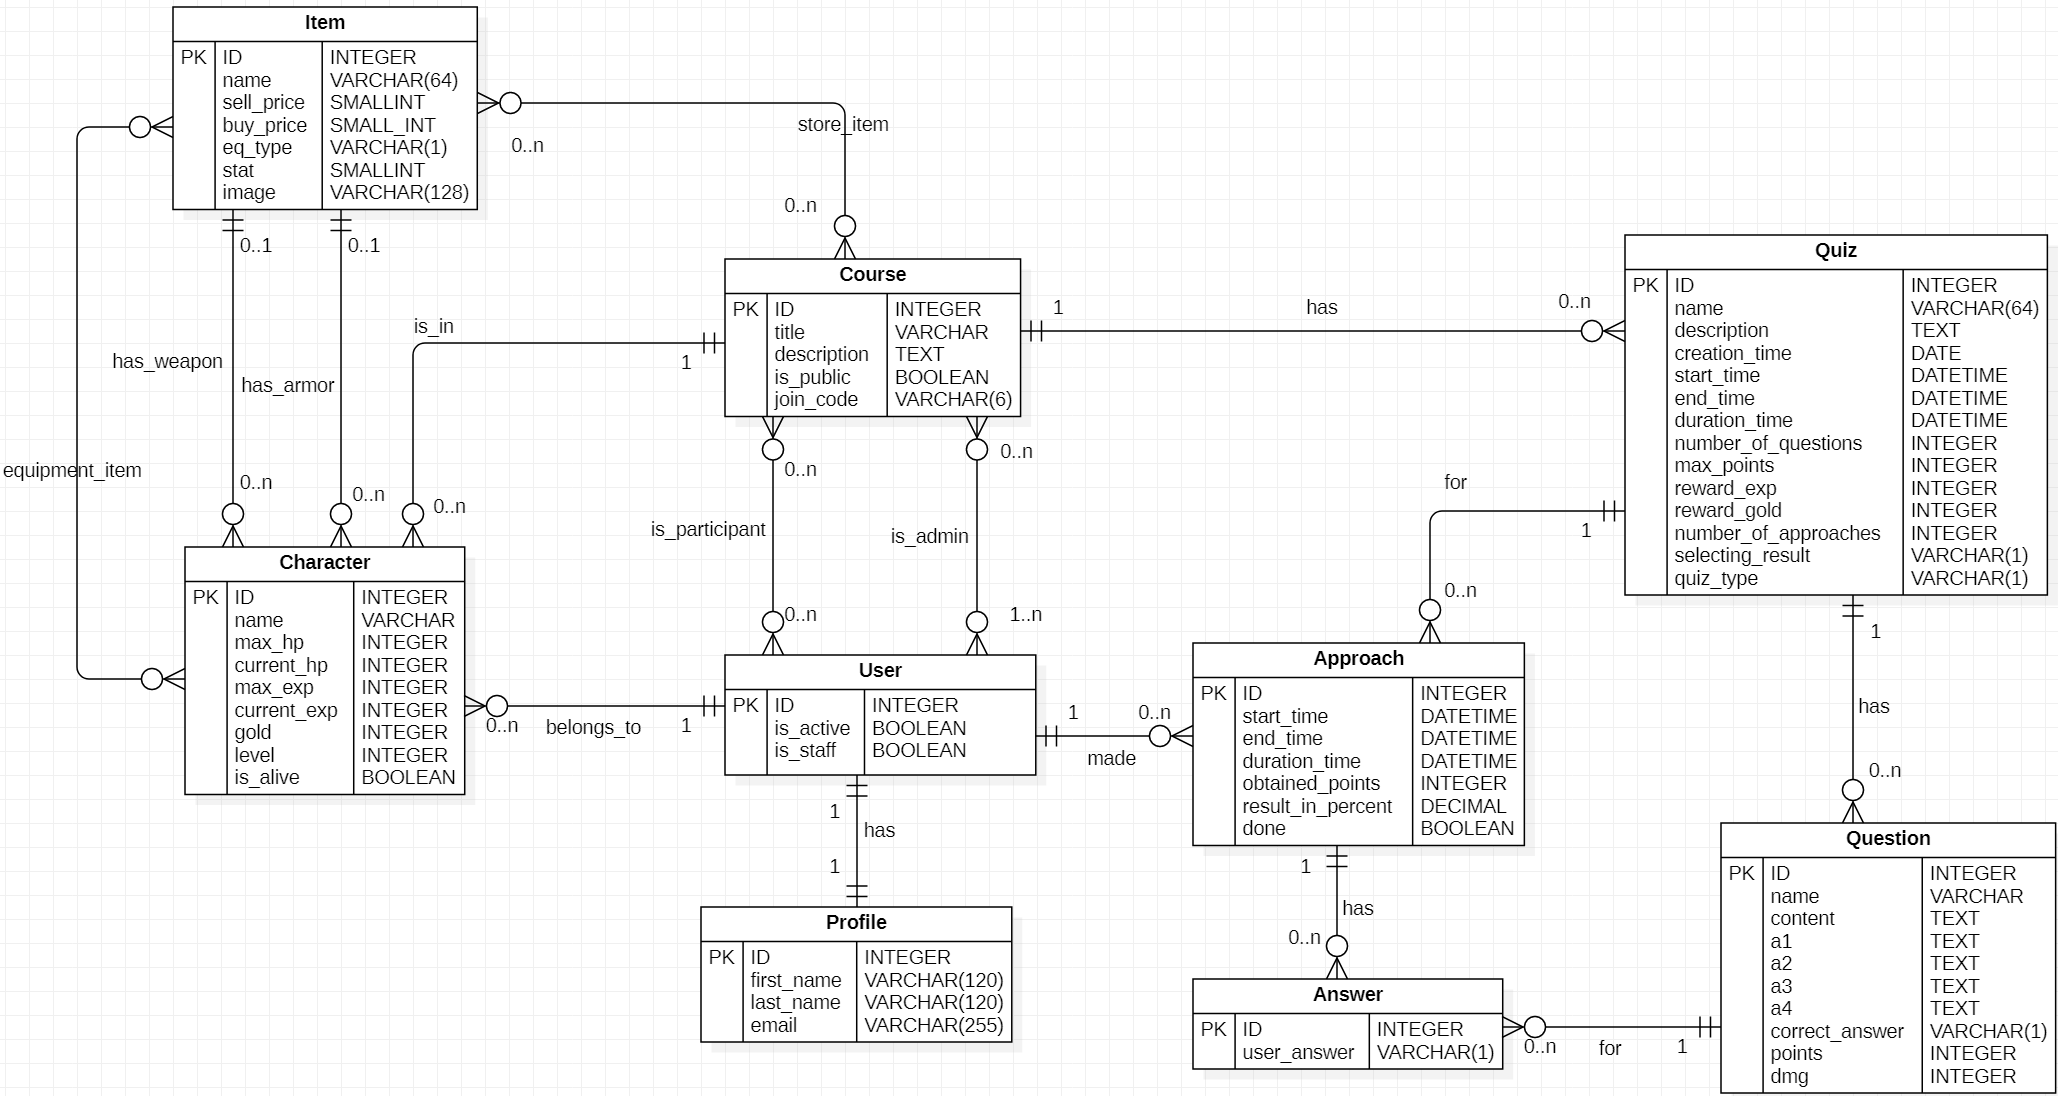
\includegraphics[width=1.6\textwidth, angle =90 ]{img/chapter5/erd_diagram.png}
	\caption{Diagram bazy danych}
	\label{chapter_5_erd}
\end{figure}

\clearpage